Convolutional Neural Networks (CNNs) are artificial neural networks mostly used in image analyzing.
Let's take a closer look on how our original CNN python script behaves. We are going to be using 
PyTorch, a deep learning framework. We utilize the following modules:
\subsection{Dependencies}
\begin{itemize}
    \item \textcolor{orange}{\textbf{torch.nn}}: Module for building neural networks
    \item \textcolor{orange}{\textbf{torch.optim}}: Module for optimization algorithms (e.g., Adam, SGD)
    \item \textcolor{orange}{\textbf{torchvision}}: Module that provides our dataset and data transformation utilities
    \item \textcolor{orange}{\textbf{DataLoader}} from \texttt{torch.utils.data}: Module for loading the dataset
\end{itemize}

Other useful libraries:
\begin{itemize}
    \item \textcolor{orange}{\textbf{matplotlib}}: Plotting and calculations
    \item \textcolor{orange}{\textbf{time}}: To measure the training duration
\end{itemize}

\begin{lstlisting}[caption={Dependencies Code}, label={lst:dependencies}]
    import torch
    import torch.nn as nn
    import torch.optim as optim
    import torchvision
    import torchvision.transforms as transforms
    import matplotlib.pyplot as plt
    from torch.utils.data import DataLoader
    import time
\end{lstlisting}

As mentioned previously, we are going to use the CIFAR-10 dataset. These are the different classes:
\begin{lstlisting}[caption={CIFAR-10 Classes}, label={lst:cifar_classes}]
    # Specify the classes
    classes = ('plane', 'car', 'bird', 'cat', 'deer', 'dog', 'frog', 'horse', 'ship', 'truck')
\end{lstlisting}

Next come the training and evaluation functions.

\subsection{Training Function}
The training process entails four basic steps:
\begin{enumerate}
    \item \textcolor{orange}{\textbf{Forward pass}}: We pass the images through the CNN neural network.
    \item \textcolor{orange}{\textbf{Loss Calculation}}: We calculate how far the model's predictions are from the ground truth.
    \item \textcolor{orange}{\textbf{Backward pass}}: We use back-propagation to compute the gradient of the loss function with respect to each weight in the network. This represents how much each weight contributed to the error.
    \item \textcolor{orange}{\textbf{Optimization}}: Using the Adam optimizer, we update the weights in order to minimize the loss.
\end{enumerate}

\begin{lstlisting}[caption={Training Function}, label={lst:training}]
    # Training function
    def train(model, trainloader, criterion, optimizer, device):
        model.train() # Set model to training mode
        running_loss = 0.0 #
        correct = 0 # Number of correctly predicted images
        total = 0 # Total number of images
        
        # Iterate over the training dataset
        for i, data in enumerate(trainloader, 0):
            inputs, labels = data[0].to(device), data[1].to(device) #data[0] is the image, data[1] is the label
            
            optimizer.zero_grad() # Reset the gradients of model parameters
            outputs = model(inputs) # Forward pass
            loss = criterion(outputs, labels) # Calculate loss
            loss.backward() # Backward pass
            optimizer.step() # Update weights
            
            # Track training statistics
            running_loss += loss.item() # Add loss to running loss
            _, predicted = outputs.max(1) # Get the class index with the highest probability
            total += labels.size(0) # Add batch size to total
            correct += predicted.eq(labels).sum().item() # Add number of correct predictions to correct
            
            # Print statistics every 100 mini-batches
            if i % 100 == 99:
                print(f'[{i + 1}] loss: {running_loss / 100:.3f} | acc: {100.*correct/total:.2f}%')
                running_loss = 0.0 # Reset running loss
        
        return 100. * correct / total
\end{lstlisting}


\subsection{Evaluation Function}
The evaluation process entails three steps:
\begin{enumerate}
    \item \textcolor{orange}{\textbf{Forward pass}}
    \item \textcolor{orange}{\textbf{Loss Calculation}}
\end{enumerate}

There is no need to \textcolor{orange}{\textbf{Backward pass}} or \textcolor{orange}{\textbf{Optimize}}
our neural network since we are only testing its final state.

\begin{lstlisting}[caption={Evaluation Function}, label={lst:evaluation}]
    # Evaluation function
    def evaluate(model, testloader, criterion, device):
    model.eval() # Set model to evaluation mode
    test_loss = 0 # Total loss
    correct = 0 # Number of correctly predicted images
    total = 0 # Total number of images
    
    # Compute per-class accuracy
    class_correct = [0]*10
    class_total = [0]*10

    with torch.no_grad(): # Disable gradient calculation
        # Iterate over the test dataset
        for data in testloader: 
            images, labels = data[0].to(device), data[1].to(device) # data[0] is the image, data[1] is the label
            outputs = model(images) # Forward pass
            loss = criterion(outputs, labels) # Calculate loss
            
            # Track test statistics
            test_loss += loss.item() # Add loss to test loss
            _, predicted = outputs.max(1) # Get the class index with the highest probability
            total += labels.size(0) # Add batch size to total
            correct += predicted.eq(labels).sum().item() # Add number of correct predictions to correct

            # Update per-class statistics
            for i in range(len(labels)):  # Loop through each image in the batch
                label = labels[i]
                class_correct[label] += (predicted[i] == label).item()  # Increment correct count for this class
                class_total[label] += 1  # Increment total count for this class

    # Calculate overall test accuracy and average loss            
    accuracy = 100. * correct / total # Calculate accuracy
    avg_loss = test_loss / len(testloader) # Calculate average loss
    print(f'Test set: Average loss: {avg_loss:.4f}, Accuracy: {accuracy:.2f}%')

    # Calculate per-class accuracy
    print('\nPer-class accuracy:')
    for i in range(10):
        if class_total[i] > 0: # Avoid division by zero
            class_accuracy = 100. * class_correct[i] / class_total[i]
            print(f'{classes[i]:>5s}: {class_accuracy:.2f}%')

    return accuracy, avg_loss
\end{lstlisting}


\subsection{CNN Model}
The CNN class defines the model architecture. There are 3 steps we have to go through:
\begin{enumerate}
    \item Convolutional layers
    \item Fully connected layers
    \item Forward pass
\end{enumerate}

\subsubsection{Convolutional Layers}
An example convolutional layer (e.g. \texttt{nn.Conv2d(3, 32, 3, padding=1)} ) has:
\begin{itemize}
    \item \textcolor{orange}{\textbf{Input}}: This is the first convolution layer, so the input is
    the function's first parameter "3". They represent an image's RGB channels. 
    \item \textcolor{orange}{\textbf{Output}}: Each neuron's output is 32 filters.
    \item \textcolor{orange}{\textbf{Filter}}: As shown in the function's third parameter, the filter 
    is a 3x3 kernel. This just means that each filter is a 3x3 matrix. It is the window that slides 
    over each 3x3 set of pixels scanning the entire input image.
    \item \textcolor{orange}{\textbf{Padding}}: The function's fourth parameter is padding. Padding 
    is used to preserve the image's dimensions even after the convolution operation.
\end{itemize}

\begin{lstlisting}[caption={CNN Model}, label={lst:cnn_model}]
    # Define the CNN architecture
    class CNN(nn.Module):
        # Initialize the architecture
        def __init__(self):
            super(CNN, self).__init__()
            self.conv_layers = nn.Sequential(
                # First convolutional layer
                nn.Conv2d(3, 32, 3, padding=1), # 3 input channels (R G B), 32 output channels, 3x3 kernel, 1 padding
                nn.BatchNorm2d(32), # normalize the output of the previous layer to have a mean = 0 and standard deviation = 1
                nn.ReLU(), # ReLU activation function: f(x) = max(0, x)

                # Second convolutional layer
                nn.Conv2d(32, 64, 3, padding=1),
                nn.BatchNorm2d(64),
                nn.ReLU(), 
                nn.MaxPool2d(2, 2),  # for each 2x2 window, take the maximum value
                nn.Dropout(0.25), # set 25% of the neurons to zero

                # Third convolutional layer
                nn.Conv2d(64, 128, 3, padding=1),
                nn.BatchNorm2d(128),
                nn.ReLU(),

                # Fourth convolutional layer
                nn.Conv2d(128, 128, 3, padding=1),
                nn.BatchNorm2d(128),
                nn.ReLU(),
                nn.MaxPool2d(2, 2),
                nn.Dropout(0.25),

                # Fifth convolutional layer
                nn.Conv2d(128, 256, 3, padding=1),
                nn.BatchNorm2d(256),
                nn.ReLU(),

                # Sixth convolutional layer
                nn.Conv2d(256, 256, 3, padding=1),
                nn.BatchNorm2d(256),
                nn.ReLU(),
                nn.MaxPool2d(2, 2),
                nn.Dropout(0.25),
            )
            # Fully connected layers
            self.fc_layers = nn.Sequential(
                nn.Linear(256 * 4 * 4, 512), # First fully connected layer
                nn.ReLU(),
                nn.Dropout(0.5),
                nn.Linear(512, 10) # Final fully connected layer, 512 input features, 10 output features (classes)
            )

        # Define the forward pass
        def forward(self, x):
            x = self.conv_layers(x) # Pass input through convolutional layers
            x = x.view(x.size(0), -1) # Flatten the output of the convolutional layers
            x = self.fc_layers(x) # Pass through fully connected layers
            return x
\end{lstlisting}

\begin{lstlisting}
    # Set random seed for reproducibility
    torch.manual_seed(42)

    # The variable "device" specifies the computational device 
    # This is where we run our neural network on (CPU or GPU)
    device = torch.device('cuda' if torch.cuda.is_available() else 'cpu')

    # Data Preprocessing 
    # Tranformations for the training dataset
    transform_train = transforms.Compose([
        transforms.RandomCrop(32, padding=4), # Randomly crops image with padding
        transforms.RandomHorizontalFlip(), # Randomly flips image horizontally
        transforms.ToTensor(), # Converts image to tensor
        transforms.Normalize((0.4914, 0.4822, 0.4465), (0.2023, 0.1994, 0.2010))
    ])
    # Tranformations for the test dataset
    transform_test = transforms.Compose([
        transforms.ToTensor(), # Converts image to tensor
        transforms.Normalize((0.4914, 0.4822, 0.4465), (0.2023, 0.1994, 0.2010))
    ])
\end{lstlisting}


\subsection{Model Initialization}
\subsubsection{Loss Function}
Calculates how well the model is doing by measuring the difference between the model's predictions and the actual target values (ground truth). The lower the loss, the better the predictions. For classification problems, we use:
\begin{itemize}
    \item \textbf{Cross-Entropy Loss}
    \begin{itemize}
        \item Measures the difference between predicted probability distributions and actual classes.
        \item Commonly used for categorizing into discrete classes.
    \end{itemize}
\end{itemize}

\subsubsection{Optimizer}
\textbf{Adam (Adaptive Moment Estimation)} is an optimization algorithm that updates the model's 
weights to minimize the loss function.

\subsubsection{Learning Rate Scheduler}
Dynamically adjusts the learning rate during training:
\begin{itemize}
    \item Reduces learning rate when performance peaks.
    \item \textbf{patience=3}: Waits for 3 epochs without improvement before triggering.
    \item \textbf{factor=0.5}: Reduces learning rate by half when triggered.
    \item \textbf{min}: Monitors a metric and reduces learning rate when it stops decreasing.
\end{itemize}

\texttt{scheduler.step(test\_loss)} \\ 
When the scheduler is called later in the code's main loop, it is set to minimize the test loss.

\textbf{Example}
\begin{enumerate}
    \item Starting Learning Rate (LR) = 0.001
    \item After plateau (no improvement for 3 epochs):
    \item New LR = $0.001 \times 0.5 = 0.0005$
    \item After another plateau:
    \item New LR = $0.0005 \times 0.5 = 0.00025$
\end{enumerate}

\begin{lstlisting}[caption={Model Initialization}, label={lst:model_init}]
    # Model Initialization
    model = CNN().to(device) # Send model to device for training
    criterion = nn.CrossEntropyLoss() # Loss function
    optimizer = optim.Adam(model.parameters(), lr=0.001) # Optimizer
    scheduler = optim.lr_scheduler.ReduceLROnPlateau(optimizer, 'min', patience=3, factor=0.5) # Learning rate scheduler
\end{lstlisting}

\subsection{Preparation}

\subsubsection{Data Preprocessing}
Transformations imposed on the training data improve generalization. The steps for preprocessing 
are as follows:
\begin{itemize}
    \item Cropping
    \item Flipping
    \item Conversion to tensor
    \item Normalization
\end{itemize}

However, during testing, we only normalize the data:
\begin{itemize}
    \item Conversion to tensor
    \item Normalization
\end{itemize}

\subsubsection{Conversion to Tensor}
\textbf{Converts the input image} into a PyTorch tensor for easy manipulation. The tensor format:
\begin{itemize}
    \item \textcolor{orange}{\textbf{Rescales}} pixel values from the range [0, 255] (for images) 
    to [0, 1] by dividing by 255.
    \item \textcolor{orange}{\textbf{Rearranges the image dimensions}} from (Height * Width * Channels)
    to (Channels * Height * Width) to match PyTorch's convention.
\end{itemize}

The Tensor format is required for performing computations in PyTorch models.

\subsubsection{Normalization}
For each channel (R, G, B), normalization subtracts the corresponding mean $(0.4914, 0.4822, 0.4465)$ 
and divides by the corresponding standard deviation $(0.2023, 0.1994, 0.2010)$:

$$\text{Normalized Value} = \frac{\text{Pixel Value} - \text{Mean}}{\text{Standard Deviation}}$$

Normalization helps standardize the input data, which improves the convergence of the model during 
training.

\subsubsection{Data Loading}
\textit{Loading dataset and applying previous transformations...}

\begin{lstlisting}[caption={Data Preparation}, label={lst:data_prep}]
    # Set random seed for reproducibility
    torch.manual_seed(42)

    # The variable "device" specifies the computational device 
    # This is where we run our neural network on (CPU or GPU)
    device = torch.device('cuda' if torch.cuda.is_available() else 'cpu')

    # Data Preprocessing 
    # Tranformations for the training dataset
    transform_train = transforms.Compose([
        transforms.RandomCrop(32, padding=4), # Randomly crops image with padding
        transforms.RandomHorizontalFlip(), # Randomly flips image horizontally
        transforms.ToTensor(), # Converts image to tensor
        transforms.Normalize((0.4914, 0.4822, 0.4465), (0.2023, 0.1994, 0.2010))
    ])
    # Tranformations for the test dataset
    transform_test = transforms.Compose([
        transforms.ToTensor(), # Converts image to tensor
        transforms.Normalize((0.4914, 0.4822, 0.4465), (0.2023, 0.1994, 0.2010))
    ])

    # Our Dataset
    # Load CIFAR-10 training dataset
    trainset = torchvision.datasets.CIFAR10(root='./cifar-10-batches-py', train=True, download=True, transform=transform_train)
    trainloader = DataLoader(trainset, batch_size=128, shuffle=True, num_workers=2)
    # Load CIFAR-10 test dataset
    testset = torchvision.datasets.CIFAR10(root='./cifar-10-batches-py', train=False, download=True, transform=transform_test)
    testloader = DataLoader(testset, batch_size=100, shuffle=False, num_workers=2)
\end{lstlisting}

\subsection{Training Loop}
This is the main loop of the training process. Here, we utilize the aforementioned functions to:
\begin{itemize}
    \item \textcolor{orange}{\textbf{Train}}: Train the neural network on the dataset.
    \item \textcolor{orange}{\textbf{Evaluate}}: Test the neural network's performance.
    \item \textcolor{orange}{\textbf{Benchmark}}: Compare the performance of the model.
    \item \textcolor{orange}{\textbf{Save}}: Save the trained neural network's weights for future use.
\end{itemize}

\begin{lstlisting}[caption={Training Loop}, label={lst:training_loop}]
    # Main loop
    num_epochs = 50 # Number of epochs
    best_acc = 0 # Best accuracy
    train_acc_history = [] # Training accuracy history
    test_acc_history = [] # Test accuracy history

    print(f"Training on {device}") # Print device
    start_time = time.time() # Start time

    # Iterate over the epochs
    for epoch in range(num_epochs):
        print(f'\nEpoch {epoch+1}/{num_epochs}') # Print epoch
        
        # Train and evaluate the model
        train_acc = train(model, trainloader, criterion, optimizer, device)
        test_acc, test_loss = evaluate(model, testloader, criterion, device)
        
        # Track accuracy history
        train_acc_history.append(train_acc)
        test_acc_history.append(test_acc)
        
        # Learning rate scheduling
        scheduler.step(test_loss) # Adjust learning rate based on loss
        
        # Save best model
        if test_acc > best_acc:
            print(f'Saving best model with accuracy: {test_acc:.2f}%') # Print current best accuracy
            # Save the model with the best accuracy in the filename
            torch.save(model.state_dict(), f'./cifar10_acc_{test_acc:.2f}.pth')
            best_acc = test_acc

    # Calculate training time
    training_time = time.time() - start_time # Calculate training time
    print(f'\nTraining completed in {training_time/60:.2f} minutes') # Print training time
    print(f'Best accuracy: {best_acc:.2f}%') # Print final best accuracy
\end{lstlisting}

\subsection{Accuracy History}
Finally plot the training history to spot the point of diminishing returns.

\begin{lstlisting}[caption={Accuracy History}, label={lst:history}]
    # Plot training history
    plt.figure(figsize=(10, 5))
    plt.plot(train_acc_history, label='Train Accuracy')
    plt.plot(test_acc_history, label='Test Accuracy')
    plt.title('Model Accuracy over Time')
    plt.xlabel('Epoch')
    plt.ylabel('Accuracy (%)')
    plt.legend()
    plt.grid(True)
    plt.savefig('cifar10_accuracy.png')
    plt.show()
\end{lstlisting}

\subsection{Results}
Since the only coding machine I had in my disposal was using an AMD GPU I couldn't utilize the
CUDA torch device to accelerate the training process. That's why I ended up uploading my program
to Aristotle's HPC (High Performance Computing) cluster to take advantage of the RTX A4000 GPU 
which was more than enough for our use case. Here are the results when choosing to train the model
for 50 epochs:
\begin{figure}[H]
    \centering
    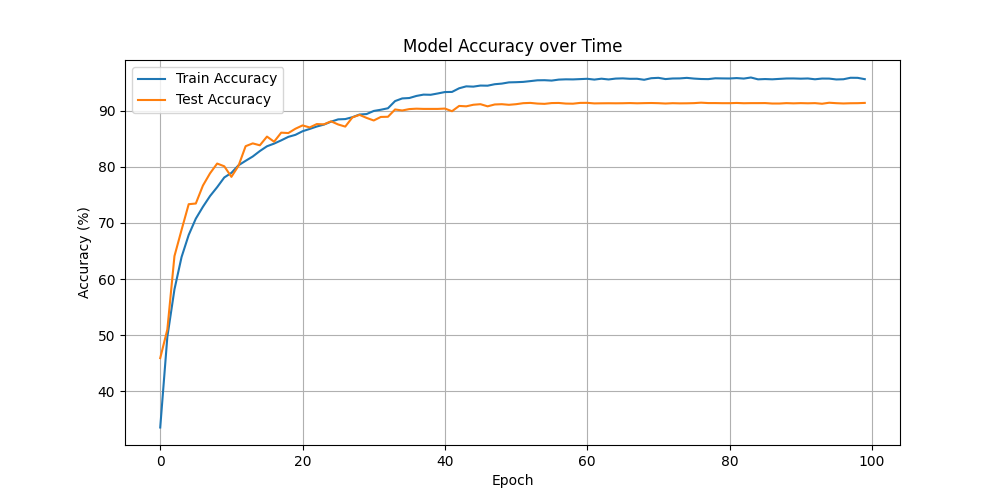
\includegraphics[width=4in]{media/cifar10_accuracy.png}
    \caption{Accuracy History}
    \label{CIFAR example}
\end{figure}
Here it is evident that around epoch 50 the model begins to settle on the final accuracy, while past
epoch 60 there is barely any fluctuation.
\begin{figure}[H]
    \centering
    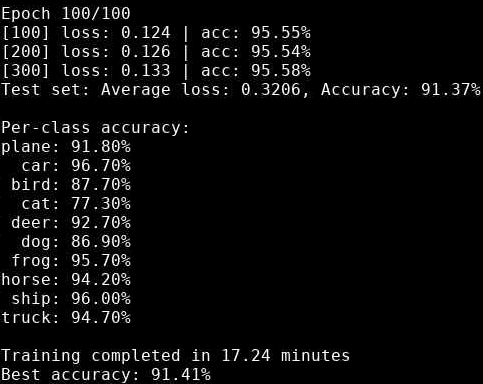
\includegraphics[width=3in]{media/epoch_100.png}
    \caption{Epoch 100 console output}
    \label{CIFAR example}
\end{figure}
As shown on the last epoch, the final accuracy when testing the emerging model is around 91\%. The 
training accuracy was around 96\%. This difference is explained by the fact that the model is better
at predicting the images that it was trained on, rather than the unseen test images. However over-fitting
doesn't seem to be an issue here. The resulting accuracies are close to one another. This is thanks to:
\begin{itemize}
    \item The dropout layers
    \item The batch normalization layers
    \item The data augmentation (random crops and horizontal flips) 
\end{itemize}

